\documentclass[a4paper,11pt]{article}
\usepackage{amsmath,amsthm,amsfonts,amssymb,amscd,amstext,vmargin,graphics,graphicx,tabularx,multicol} 
\usepackage[francais]{babel}
\usepackage[utf8]{inputenc}  
\usepackage[T1]{fontenc} 
\usepackage{pstricks-add,tikz,tkz-tab,variations}
\usepackage[autolanguage,np]{numprint} 

\setmarginsrb{1.5cm}{0.5cm}{1cm}{0.5cm}{0cm}{0cm}{0cm}{0cm} %Gauche, haut, droite, haut
\newcounter{numexo}
\newcommand{\exo}[1]{\stepcounter{numexo}\noindent{\bf Exercice~\thenumexo} : \marginpar{\hfill /#1}}
\reversemarginpar


\newcounter{enumtabi}
\newcounter{enumtaba}
\newcommand{\q}{\stepcounter{enumtabi} \theenumtabi.  }
\newcommand{\qa}{\stepcounter{enumtaba} (\alph{enumtaba}) }
\newcommand{\initq}{\setcounter{enumtabi}{0}}
\newcommand{\initqa}{\setcounter{enumtaba}{0}}

\newcommand{\be}{\begin{enumerate}}
\newcommand{\ee}{\end{enumerate}}
\newcommand{\bi}{\begin{itemize}}
\newcommand{\ei}{\end{itemize}}
\newcommand{\bp}{\begin{pspicture*}}
\newcommand{\ep}{\end{pspicture*}}
\newcommand{\bt}{\begin{tabular}}
\newcommand{\et}{\end{tabular}}
\renewcommand{\tabularxcolumn}[1]{>{\centering}m{#1}} %(colonne m{} centrée, au lieu de p par défault) 
\newcommand{\tnl}{\tabularnewline}

\newcommand{\trait}{\noindent \rule{\linewidth}{0.2mm}}
\newcommand{\hs}[1]{\hspace{#1}}
\newcommand{\vs}[1]{\vspace{#1}}

\newcommand{\N}{\mathbb{N}}
\newcommand{\Z}{\mathbb{Z}}
\newcommand{\R}{\mathbb{R}}
\newcommand{\C}{\mathbb{C}}
\newcommand{\Dcal}{\mathcal{D}}
\newcommand{\Ccal}{\mathcal{C}}
\newcommand{\mc}{\mathcal}

\newcommand{\vect}[1]{\overrightarrow{#1}}
\newcommand{\ds}{\displaystyle}
\newcommand{\eq}{\quad \Leftrightarrow \quad}
\newcommand{\vecti}{\vec{\imath}}
\newcommand{\vectj}{\vec{\jmath}}
\newcommand{\Oij}{(O;\vec{\imath}, \vec{\jmath})}
\newcommand{\OIJ}{(O;I,J)}


\newcommand{\bmul}[1]{\begin{multicols}{#1}}
\newcommand{\emul}{\end{multicols}}

\newcommand{\reponse}[1][1]{%
\multido{}{#1}{\makebox[\linewidth]{\rule[0pt]{0pt}{20pt}\dotfill}
}}

\newcommand{\titre}[5] 
% #1: titre #2: haut gauche #3: bas gauche #4: haut droite #5: bas droite
{
\noindent #2 \hfill #4 \\
#3 \hfill #5

\vspace{-1.6cm}

\begin{center}\rule{6cm}{0.5mm}\end{center}
\vspace{0.2cm}
\begin{center}{\large{\textbf{#1}}}\end{center}
\begin{center}\rule{6cm}{0.5mm}\end{center}
}



\begin{document}
\pagestyle{empty}
\titre{Correction de l'interrogation : Outils pour la physique}{Nom :}{Prénom :}{Classe}{Date}




\exo{2}  Quels sont les graphiques où la température est proportionnelle au temps ? (Justifier votre réponse)\\

\includegraphics[scale=1.2]{graphiqueproporionnalite.eps} \\


\color{red}
Les graphiques où la température est proportionnelle au temps sont le graphique 1 et le graphique 4. Dans ces 2 graphiques, la représentation graphique est une droite qui passe par l'origine du repère.\\


\color{black}




\exo{3} Une famille a effectué une randonnée en montagne. Le graphique ci-dessous donne la distance parcourue en km en fonction du temps en heures.\\



\includegraphics[scale=0.7]{graphiquelecture.eps} 
\initq



\textit{ On utilisera le graphique pour répondre aux questions suivantes. Aucune justification n'est
demandée.} \\
\q \qa Quelle distance cette famille a-t-elle parcourue au total ?\\
\color{red}
Au total, la famille aura parcourue 20 km.\\
\color{black}


\qa Quelle est la distance parcourue au bout de 3 h de marche ?\\
\color{red}
Au bout de 6h de  marche, la famille a parcouru 8 km.\\
\color{black}




\q Y a-t-il proportionnalité entre la distance parcourue et la durée de parcours de cette étape ? Justifier votre réponse.\\
\color{red}
La représentation graphique de ce parcours n'est pas une droite donc il n'y a pas proportionnalité entre la distance parcourue et la durée de parcours de cette étape.\\
\color{black}


\newpage


\exo{2} Une entreprise a produit 300 tonnes d'écrous et de vis. Elle a vendu un quart de sa production sur le marché national, 50 \% sur le marché européen, 10 \% sur le marché américain et le reste sur le marché asiatique.\\

Dans chaque cas, calculer la masse d'écrous (en tonnes) vendue.\\
\color{red}

Marché national : $\dfrac{1}{4} \times 300 = 75$ tonnes d'écrous et de vis vendues\\

Marché européen : $\dfrac{50}{100} \times 300 = 150$ tonnes d'écrous et de vis vendues\\

Marché américain : $\dfrac{10}{100} \times 300 = 30$ tonnes d'écrous et de vis vendues\\

Marché asiatique : 300 - 75 - 150 - 30 = 45 tonnes d'écrous et de vis vendues\\

\color{black}



\exo{2} Compléter avec l'écriture décimale ou bien la puissance de dix correspondante  :

\bmul{4}

$10^{2} = $ \textcolor{red}{100}
\columnbreak


\textcolor{red}{$10^{3} $ }= 1 000

\columnbreak

$10^{5} = $ \textcolor{red}{100 000}
\columnbreak


\textcolor{red}{$10^{8}  $} = 100 000 000 

\emul





\exo{3} Voici 4 objets de l'univers :\\

\begin{tabular}{|c|c|c|c|}
\hline 
\includegraphics[scale=0.3]{terre.eps}  & \includegraphics[scale=0.3]{tour.eps} & \includegraphics[scale=0.2]{galaxie.eps} & \includegraphics[scale=0.2]{systeme.eps}  \\ 
\hline 
La Terre & La plus haute tour du monde & La galaxie & Le système solaire  \\ 
\hline
\end{tabular} 


\vspace*{0.5cm}
Voici les dimensions approximatives de ces 4 objets :\\

\begin{tabular}{|c|c|c|c|}
\hline 
\hspace*{0.5cm}828 m  \hspace*{0.5cm}& \hspace*{0.5cm}12 750 000 m \hspace*{0.5cm}&\hspace*{0.5cm} $ 12 \times 10^{12} $ m \hspace*{0.5cm}& \hspace*{0.5cm} $10^{21}$ m \hspace*{0.5cm}\\ 
\hline 
\end{tabular} 

\vspace*{0.5cm}
\initq 
\q Associer chaque objet à sa dimension.\\
\color{red}
La Terre : 12 750 000 m\\

La plus haute tour du monde : 828 m\\

Le système solaire :$ 12 \times 10^{12} $ m\\

La galaxie : $10^{21}$ m




\color{black}

\q Pour pouvoir comparer des objets, les physiciens utilisent les distances en écriture scientifique.\\
Donner l'écriture scientifique de la dimension  de ces 4 objets.\\

\color{red}
La Terre : 12 750 000 m = $1,275\times 10^{7}$m\\

La plus haute tour du monde : 828 m =$8,28 \times 10^{2}$m\\

Le système solaire :$ 12 \times 10^{12} $ m=$1,2 \times 10^{13}$m\\

La galaxie : $10^{21}$ m = $1,0 \times 10^{21}$

\color{black}

\q Classer les dimensions de ces objets dans l'ordre croissant.\\

\color{red}
$8,28 \times 10^{2}<1,275\times 10^{7}<1,2 \times 10^{13}<1,0 \times 10^{21}$\\

La tour puis La Terre puis le système solaire puis la galaxie.\\

\color{black}





\end{document}
